\documentclass[11pt,a4paper]{article}
\usepackage[margin=2.2cm]{geometry}
\usepackage{amsmath,amssymb}
\usepackage{siunitx}
\usepackage{booktabs}
\usepackage{xcolor}
\usepackage{microtype}
\usepackage{enumitem}
\usepackage{tcolorbox}
\usepackage{graphicx}
\definecolor{ink}{HTML}{14231B}\definecolor{accent}{HTML}{0F3D2A}
\tcbuselibrary{skins}
\newtcolorbox{key}{colback=accent!6,colframe=accent,boxrule=0.6pt,arc=2pt,left=6pt,right=6pt,top=4pt,bottom=4pt}
\sisetup{per-mode=symbol,group-separator={\,}}
\setlength{\parindent}{0pt}\setlength{\parskip}{6pt}
\renewcommand{\arraystretch}{1.25}

\title{\textbf{Slide 10: power and rails}\\\large 3.3 V from the PMOD alone, split by current links}
\author{ADS7057 test board v3 \quad ---\quad study notes}\date{}
\begin{document}\maketitle\vspace{-1.2em}
\section{The power tree}
\begin{center}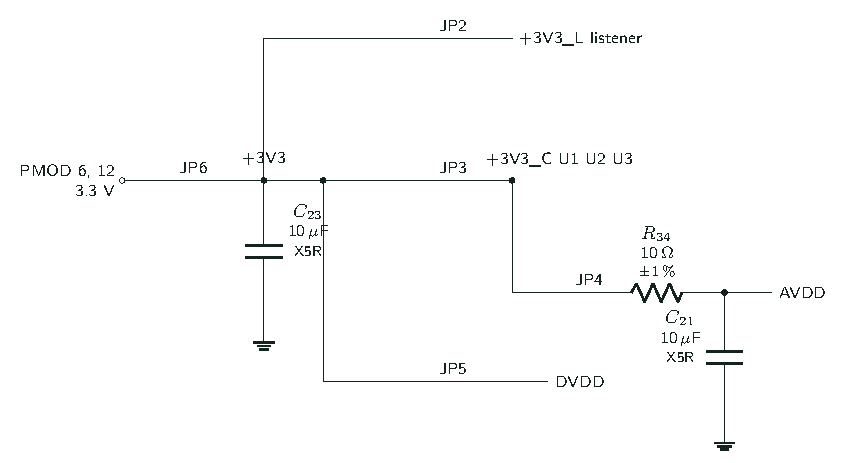
\includegraphics[width=0.98\textwidth]{s10_circuit.pdf}\end{center}
PMOD pins 6 and 12 bring 3.3 V. There is no regulator, no diode and no USB. JP6 joins the PMOD to the board rail +3V3. To run on the bench, cut JP6 and feed the 2-pin header J7 (never both). Four solder jumpers split the rail so each block can be measured alone: JP2 listener, JP3 capture chain (U1, U2, U3), JP4 ADC reference path (AVDD), JP5 ADC logic (DVDD). Cut one with a knife and put an ammeter across the gap. All four are closed at delivery.

\section{AVDD is the reference}
The ADS7057 uses AVDD as its reference, so noise on AVDD is noise in the code. AVDD comes from the rail through R34 ($10\,\Omega$) and C21 ($10\,\mu$F). First-order RC:
\[
f_c=\frac1{2\pi R_{34}C_{21}}=\frac{1}{2\pi\cdot10\,\Omega\cdot10\,\mu\text{F}}=\SI{1.59}{kHz}
\]
\[
|H(\SI{250}{kHz})|=\frac1{\sqrt{1+(250/1.59)^2}}=\frac1{157}=-43.9\ \text{dB}.
\]
\begin{center}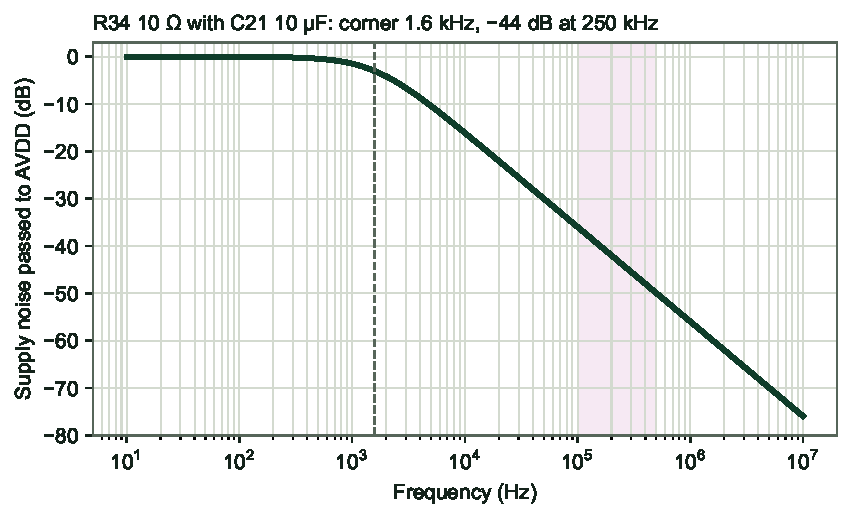
\includegraphics[width=0.6\textwidth]{s10_avdd.pdf}\end{center}
C18 ($4.7\,\mu$F) and C22 (\SI{100}{nF}) sit at the ADC pin. The DC drop over R34 is small: the ngspice rail shows AVDD at \SI{3.271}{V} against \SI{3.299}{V} on +3V3.

\section{The two mid-rails}
VMID5 (the 1.65 V that the filters and the gain stage reference) is a divider R7, R8 ($2\times10\,$k$\Omega$ from +3V3\_C) with C7 ($1\,\mu$F), copied by U2B and filtered by R9 and C8. The divider and C7 give $\tau=(R_7\parallel R_8)C_7=5\,\text{k}\Omega\times1\,\mu\text{F}=\SI{5}{ms}$, so VMID5 needs about $5\tau=\SI{25}{ms}$ after power-up. VOCM (the driver's centre) is a second divider R14, R15 ($2\times1\,$k$\Omega$ from AVDD) with C13. It follows AVDD by ratio, as the datasheet asks (AVDD/2 $\pm0.1$ V). ngspice: VMID5 1.649 V, VOCM 1.636 V.

\section{Current budget}
\begin{center}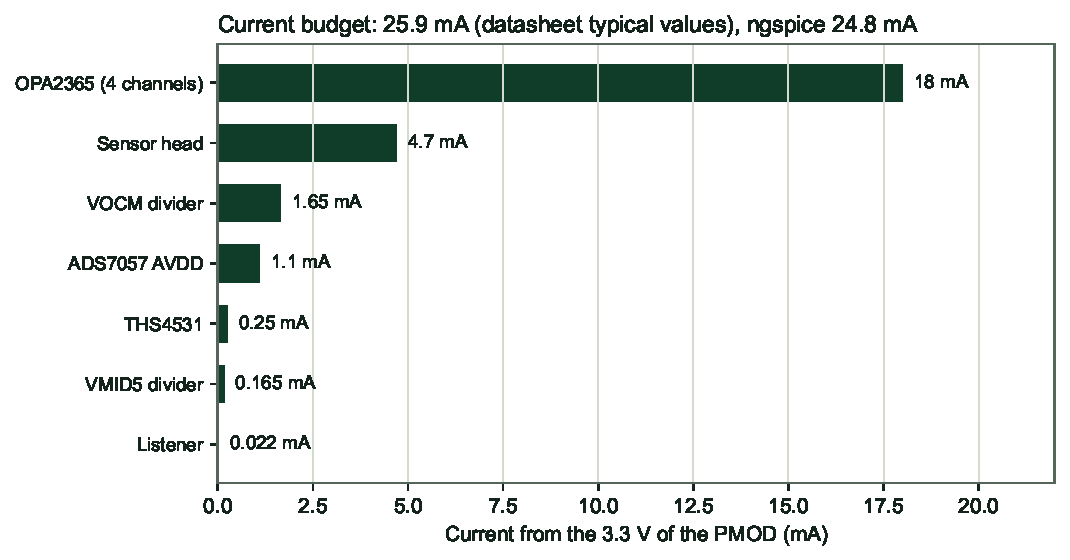
\includegraphics[width=0.85\textwidth]{s10_graph.pdf}\end{center}
The sum of the datasheet typical values is \SI{25.9}{mA}, which is \SI{85}{mW} at 3.3 V. The ngspice netlist with all links closed gives \SI{24.8}{mA}. The four OPA2365 channels dominate. The listener takes only \SI{22}{\micro A}. The 1.65 mA of the VOCM divider is the cheapest saving if the board ever runs from a battery (use $10\,$k$\Omega$ and a larger C13).

\begin{key}
Open item: the noise of the ZedBoard 3.3 V rail is not measured. Probe TP11 (+3V3) and TP12 (AVDD) on the first board.
\end{key}
\end{document}
